\documentclass[11pt]{article}
\usepackage[english]{babel}
\usepackage[utf8]{inputenc}
\usepackage[left=1cm,right=1cm,top=1cm,bottom=1.2cm]{geometry}
\usepackage{amsmath}
\usepackage{amssymb}
\usepackage{graphicx}
\usepackage{tcolorbox}
\usepackage{indentfirst}
\usepackage{hyperref}

\graphicspath{ {./images/} }

\title{\underline{IVR Coursework}}
\author{Matt Timmons-Brown \& Neil Weidinger}

\begin{document}
\maketitle

Neil and Matt worked on this coursework collaboratively - answering all questions and coding together. Thus there was an equal contribution from both members of the team.

Access the GitHub link to our code here: \url{https://github.com/the-raspberry-pi-guy/IVR-Assignment}

\setcounter{section}{1}
\section{Robot Vision}

\subsection{Joint State Estimation}

The algorithm for joint state estimation is implemented over \texttt{image1.py}, \texttt{image2.py} and \texttt{joint\_target\_estimation.py}. Each of the image files subscribe to the orthogonal camera raw data streams that are pointed at the robot in Gazebo, and thus give a view of the x/z and y/z planes respectively. 

When an image is received from the camera, the data from the image is passed to the callback - colour-based computer vision is then applied to detect each of the (different colour) joints of the robot. To achieve this, we used OpenCV colour masking, image dilation and then calculated the appropriate moment for the x/z or y/z coordinate pair, which are then published. Occasionally, a joint is obstructed by another joint/link or one of the orbiting targets. When this happens, our algorithm detects that it is occluded and uses the last known value of that joint's position.

\texttt{joint\_target\_estimation.py} receives these coordinates and, as the cameras can be assumed to be orthogonal (according to Prof Khadem live class), the x/z and y/z coordinates for all joints can be combined to form an $[x,y,z]$ vector that represents the location of the joint in 3D space.

From this, the vectors between each link of the robot are determined (ie: the blue-green link is the blue vector minus the green vector). The arctan2 operator between the blue-green vector's y and z coordinates is then used to calculate the angle for joint 2. After this, a rotation operation with a rotation matrix around the x axis is applied to rotate the blue-green vector into the newly oriented x-axis frame. Joint 3 is then calculated with arctan2 between the rotated blue-green vector's x and z coordinates. Finally, joint 4 is calculated by applying arctan2 to the green-red joint vector's y and z coordinates, and then subtracting the joint 2 angle previously calculated - as these are in the same direction (x).

Even though the cameras are orthogonal, they are not orthographic views of the world, and have a perspective effect (known as a pinhole view). This is a source of small error in our measurements and a limitation of this method. This error is observed at extreme values of the end effector.

\begin{center}
    \begin{tabular}{ll}
        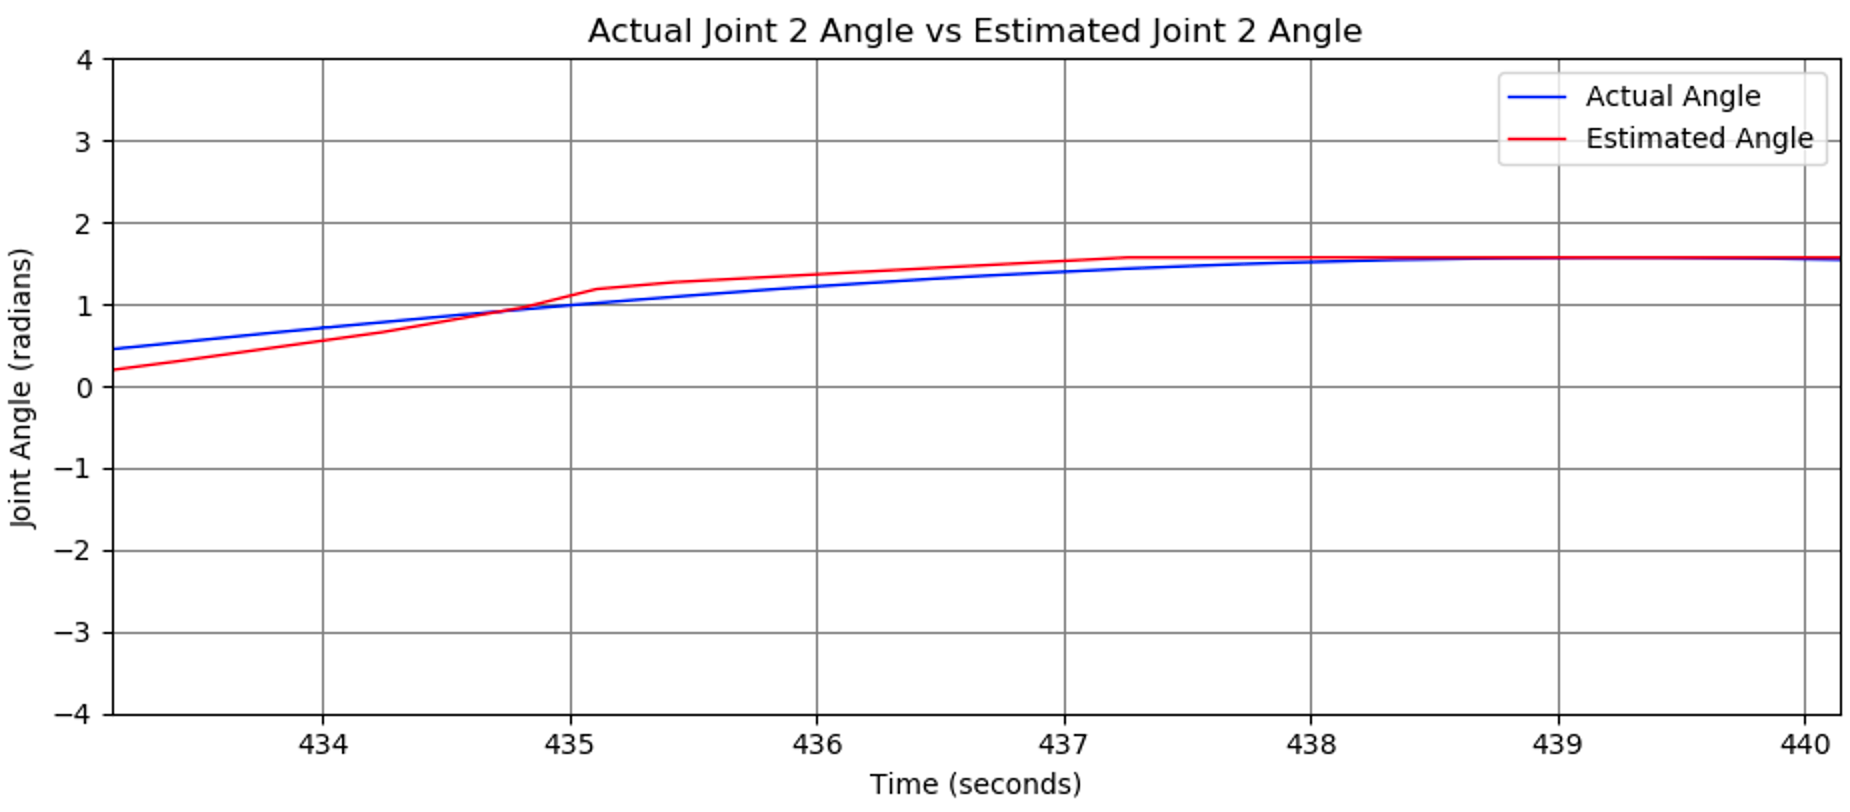
\includegraphics[width=0.4\textwidth]{images/2.1_joint2.png}
        &
        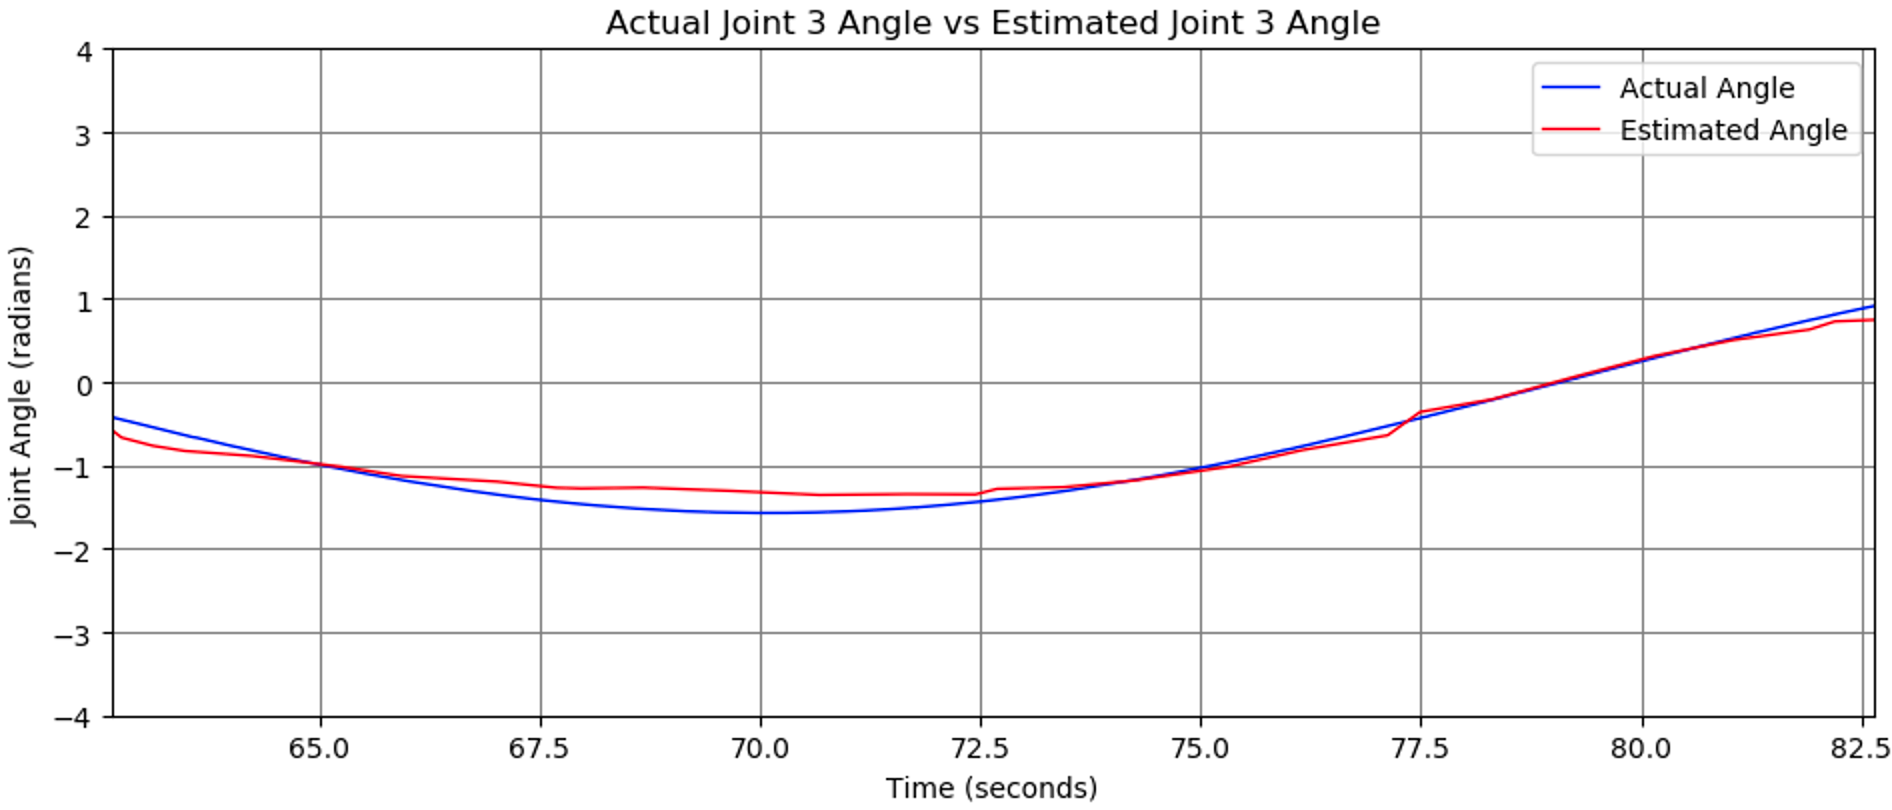
\includegraphics[width=0.4\textwidth]{images/2.1_joint3.png}
    \end{tabular}
    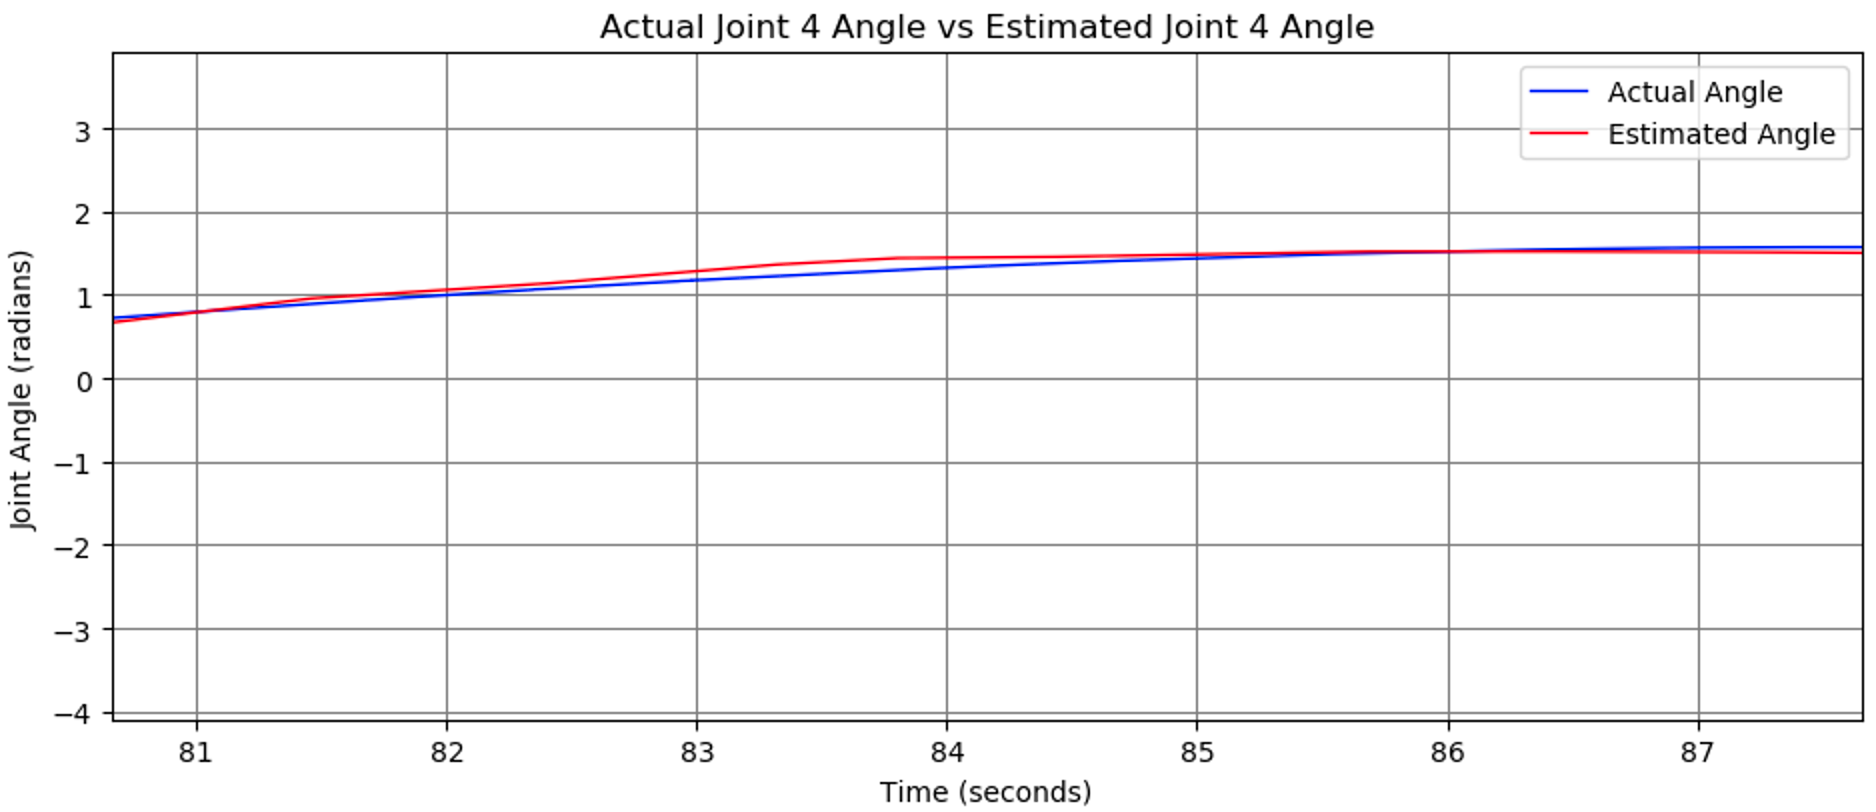
\includegraphics[width=0.4\textwidth]{images/2.1_joint4.png}
\end{center}

\subsection{Target Detection}
Similar to Q2.1, the algorithm for detection of the target sphere is distributed over the 3 files previously discussed. Crucially, there is further image processing in the \texttt{image1.py} and \texttt{image2.py} files in order to identify the sphere specifically (as it is the same colour as the cube).

As before, when an image is received from a camera, the callback triggers a detection algorithm. This disregards the bottom half of the image (as the sphere and cube never appear here) and then creates a mask with the orange shapes cut out. The contours of these shapes are then found using OpenCV, and the number of sides of the shape are identified by approximating a polygon to each shape with the OpenCV implementation of the Douglas-Peucker algorithm. As this algorithm approximates a polygon, an approximated sphere shape will be a polygon with many sides. From this we safely assume the shape with the most sides is the sphere, as the cube only ever has approximately 4 sides according to our CV testing. 

The moment of this shape is then calculated as before, and this happens in each camera to provide x/z and y/z coordinates as described in Q2.1. These are combined as before to form a $[x,y,z]$ estimate of the pixel location of the target sphere. Finally, a pixels-to-metres operation is performed to convert the pixel location to a metre-location with respect to the robot base frame. A scaling factor is calculated by counting the number of pixels between the base and first joint of the robot, and then dividing this by the known length (2.5m) of this link. We later hard coded this scaling factor for quick conversion of values, avoiding recomputation on every callback/frame.

There are a few sources of error in our measurements. Most notably, occasionally the target sphere is occluded by the robot from the perspective of one of the camera's viewpoints (ie when it orbits behind the robot). This can momentarily cause our algorithm to theoretically identify the cube as the sphere target. In practice we never observed this happening significantly. Similar to as discussed in Q2.1, the other main source of error comes from the perspective view of each camera and how it is not an orthographic view that would result in a perfectly determined $[x,y,z]$.

\begin{center}
    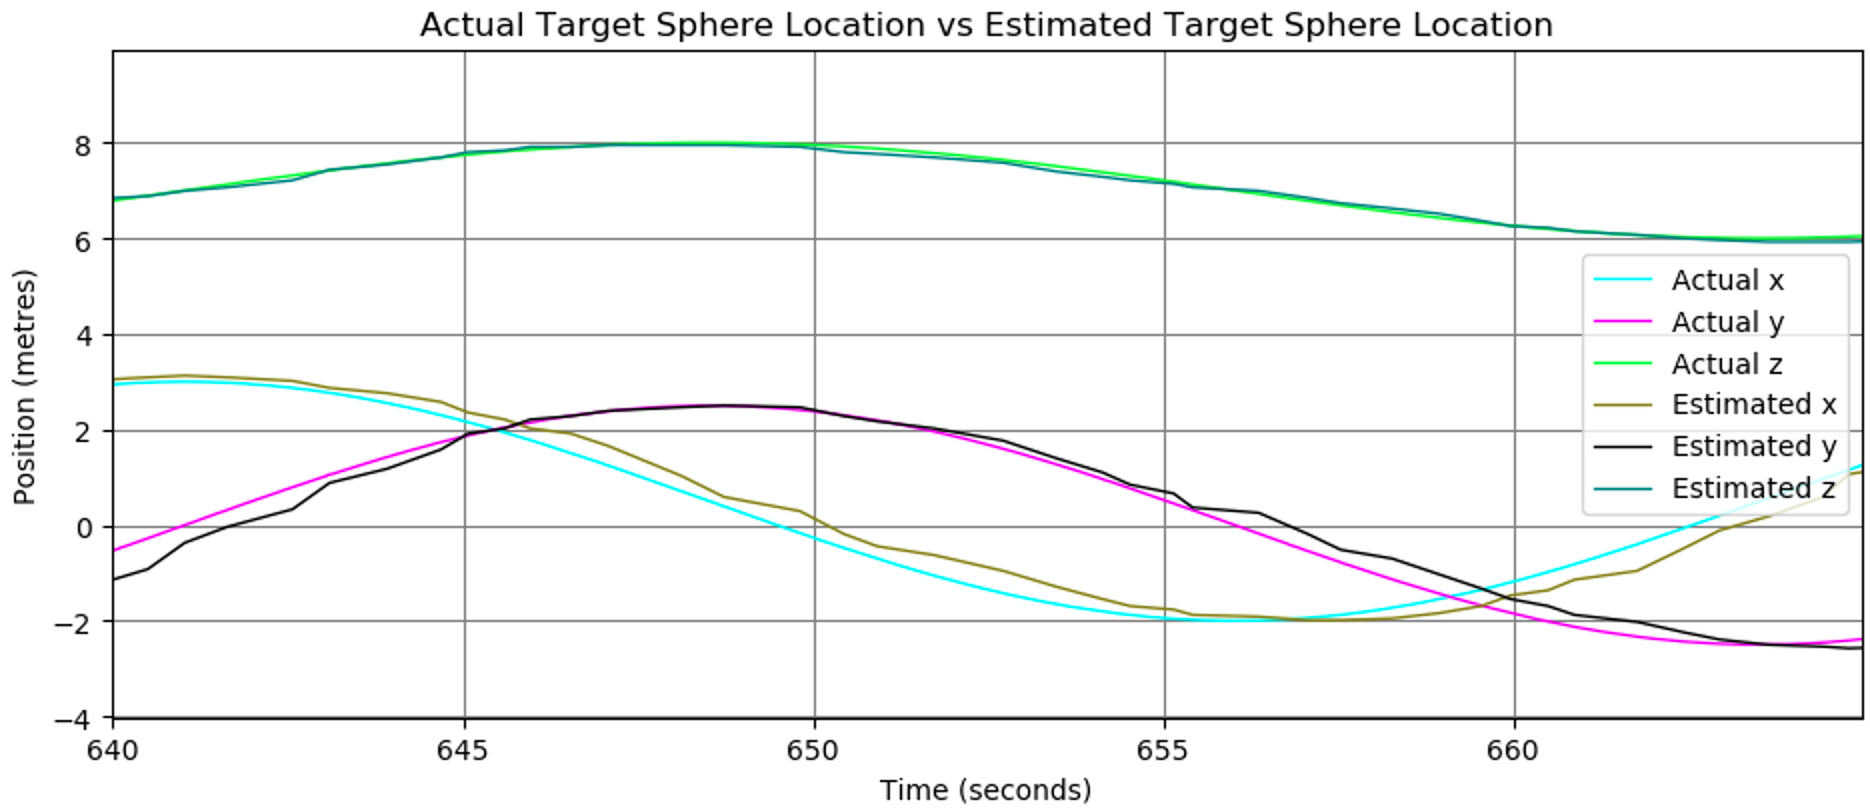
\includegraphics[width=0.4\textwidth]{images/2.2_target.png}
\end{center}

\section{Robot Control}
\subsection{Forward Kinematics}

Insert table of DH params?

\begin{center}
    \[K(q)=\left[\begin{matrix}3 s{\left(\theta_{1} \right)} s{\left(\theta_{2} \right)} c{\left(\theta_{3} \right)} c{\left(\theta_{4} \right)} + 3.5 s{\left(\theta_{1} \right)} s{\left(\theta_{2} \right)} c{\left(\theta_{3} \right)} + 3 s{\left(\theta_{1} \right)} s{\left(\theta_{4} \right)} c{\left(\theta_{2} \right)} + 3 s{\left(\theta_{3} \right)} c{\left(\theta_{1} \right)} c{\left(\theta_{4} \right)} + 3.5 s{\left(\theta_{3} \right)} c{\left(\theta_{1} \right)}\\3 s{\left(\theta_{1} \right)} s{\left(\theta_{3} \right)} c{\left(\theta_{4} \right)} + 3.5 s{\left(\theta_{1} \right)} s{\left(\theta_{3} \right)} - 3 s{\left(\theta_{2} \right)} c{\left(\theta_{1} \right)} c{\left(\theta_{3} \right)} c{\left(\theta_{4} \right)} - 3.5 s{\left(\theta_{2} \right)} c{\left(\theta_{1} \right)} c{\left(\theta_{3} \right)} - 3 s{\left(\theta_{4} \right)} c{\left(\theta_{1} \right)} c{\left(\theta_{2} \right)}\\- 3 s{\left(\theta_{2} \right)} s{\left(\theta_{4} \right)} + 3 c{\left(\theta_{2} \right)} c{\left(\theta_{3} \right)} c{\left(\theta_{4} \right)} + 3.5 c{\left(\theta_{2} \right)} c{\left(\theta_{3} \right)} + 2.5\end{matrix}\right]\]

    Where $c(\theta_i)=\cos(\theta_i)$, $s(\theta_i)=\sin(\theta_i)$
    \vspace{4mm}

    End Effector Position for Varying Joint Angles

    \begin{tabular}{|c|c|c|}
        \hline
        Joint Angle & Estimated via FK & Estimated via Images \\
        \textit{Joint 1,2,3,4 (rad)} & \textit{x,y,z (m)} & \textit{x,y,z (m)} \\ \hline
        1,0.5,0.1,-1 & 0.47,0.31,8.18 & 0.33,0.33,8.76 \\
        -1,-1,-1,1 & -1.52,4.15,6.12 & -1.36,3.68,6.59 \\
        0.25,0.25,0.25,0.25 & 2.09, -1.79, 8.33 & 2.24,-2.06,9.16 \\
        1,1,0.5,0.5 & 6.05,-0.39,4.20 & 6.11,-0.59,4.64 \\
        -1,-0.5,-0.1,1 & 4.20,2.09,5.76 & 3.68,2.72,6.22 \\
        1,1,1,-1 & 3.14,3.10,6.12 & 2.54,3.72,6.77 \\
        -0.25,-0.25,-0.25,-0.25 & -0.98,2.58,8.33 & -0.92,2.43,8.65 \\
        -1,-1,-0.5,-0.5 & 2.88,5.34,4.20 & 2.13,6.33,4.97 \\
        \(\pi\), $\pi/2$, $\pi/4$, $-0.1$ & -4.58,4.59,2.80 & -3.72,3.64,3.86 \\
        \(-\pi\), $-\pi/2$, $-\pi/4$, $0.1$ & 4.59,-4.58,2.80 & 6.07,-6.15,2.43 \\
        \hline
    \end{tabular}
\end{center}

In general, the $[x,y,z]$ positions estimated by the FK and through the computer vision roughly agree with each other (have the same signs and are of similar magnitude). However, there is a discrepancy between these values, especially at robot joint configurations where the end effector is positioned far away from the z axis. The main reason for this discrepancy is again due to the pinhole perspective view given by the cameras and the corresponding errors this introduces to the estimated $[x,y,z]$ values for the computer vision. Consequently, it is our belief that the the FK values presented in this table are of higher accuracy. This could be verified with orthographic camera views instead of the current camera setup - this would provide a more accurate computer vision estimate. Another thing to note is that the FK values are theoretically perfect, whereas the computer vision is only a practical estimate of reality, where different components can introduce real world errors (such as colour masking problems, lighting issues, etc.).

\subsection{Closed-Loop Control}

\begin{center}
    \textbf{$A =$}
    \[\left[\begin{matrix}- 3 s{\left(\theta_{1} \right)} s{\left(\theta_{3} \right)} c{\left(\theta_{4} \right)} - 3.5 s{\left(\theta_{1} \right)} s{\left(\theta_{3} \right)} + 3 s{\left(\theta_{2} \right)} c{\left(\theta_{1} \right)} c{\left(\theta_{3} \right)} c{\left(\theta_{4} \right)} + 3.5 s{\left(\theta_{2} \right)} c{\left(\theta_{1} \right)} c{\left(\theta_{3} \right)} + 3 s{\left(\theta_{4} \right)} c{\left(\theta_{1} \right)} c{\left(\theta_{2} \right)}\\3 s{\left(\theta_{1} \right)} s{\left(\theta_{2} \right)} c{\left(\theta_{3} \right)} c{\left(\theta_{4} \right)} + 3.5 s{\left(\theta_{1} \right)} s{\left(\theta_{2} \right)} c{\left(\theta_{3} \right)} + 3 s{\left(\theta_{1} \right)} s{\left(\theta_{4} \right)} c{\left(\theta_{2} \right)} + 3 s{\left(\theta_{3} \right)} c{\left(\theta_{1} \right)} c{\left(\theta_{4} \right)} + 3.5 s{\left(\theta_{3} \right)} c{\left(\theta_{1} \right)}\\0\end{matrix}\right]\]

    \textbf{$B =$}
    \[\left[\begin{matrix}- 3 s{\left(\theta_{1} \right)} s{\left(\theta_{2} \right)} s{\left(\theta_{4} \right)} + 3 s{\left(\theta_{1} \right)} c{\left(\theta_{2} \right)} c{\left(\theta_{3} \right)} c{\left(\theta_{4} \right)} + 3.5 s{\left(\theta_{1} \right)} c{\left(\theta_{2} \right)} c{\left(\theta_{3} \right)}\\3 s{\left(\theta_{2} \right)} s{\left(\theta_{4} \right)} c{\left(\theta_{1} \right)} - 3 c{\left(\theta_{1} \right)} c{\left(\theta_{2} \right)} c{\left(\theta_{3} \right)} c{\left(\theta_{4} \right)} - 3.5 c{\left(\theta_{1} \right)} c{\left(\theta_{2} \right)} c{\left(\theta_{3} \right)}\\- 3 s{\left(\theta_{2} \right)} c{\left(\theta_{3} \right)} c{\left(\theta_{4} \right)} - 3.5 s{\left(\theta_{2} \right)} c{\left(\theta_{3} \right)} - 3 s{\left(\theta_{4} \right)} c{\left(\theta_{2} \right)}\end{matrix}\right]\]

    \textbf{$C =$}
    \[\left[\begin{matrix}- 3 s{\left(\theta_{1} \right)} s{\left(\theta_{2} \right)} s{\left(\theta_{3} \right)} c{\left(\theta_{4} \right)} - 3.5 s{\left(\theta_{1} \right)} s{\left(\theta_{2} \right)} s{\left(\theta_{3} \right)} + 3 c{\left(\theta_{1} \right)} c{\left(\theta_{3} \right)} c{\left(\theta_{4} \right)} + 3.5 c{\left(\theta_{1} \right)} c{\left(\theta_{3} \right)}\\3 s{\left(\theta_{1} \right)} c{\left(\theta_{3} \right)} c{\left(\theta_{4} \right)} + 3.5 s{\left(\theta_{1} \right)} c{\left(\theta_{3} \right)} + 3 s{\left(\theta_{2} \right)} s{\left(\theta_{3} \right)} c{\left(\theta_{1} \right)} c{\left(\theta_{4} \right)} + 3.5 s{\left(\theta_{2} \right)} s{\left(\theta_{3} \right)} c{\left(\theta_{1} \right)}\\- 3 s{\left(\theta_{3} \right)} c{\left(\theta_{2} \right)} c{\left(\theta_{4} \right)} - 3.5 s{\left(\theta_{3} \right)} c{\left(\theta_{2} \right)}\end{matrix}\right]\]

    \textbf{$D =$}
    \[\left[\begin{matrix}- 3 s{\left(\theta_{1} \right)} s{\left(\theta_{2} \right)} s{\left(\theta_{4} \right)} c{\left(\theta_{3} \right)} + 3 s{\left(\theta_{1} \right)} c{\left(\theta_{2} \right)} c{\left(\theta_{4} \right)} - 3 s{\left(\theta_{3} \right)} s{\left(\theta_{4} \right)} c{\left(\theta_{1} \right)}\\- 3 s{\left(\theta_{1} \right)} s{\left(\theta_{3} \right)} s{\left(\theta_{4} \right)} + 3 s{\left(\theta_{2} \right)} s{\left(\theta_{4} \right)} c{\left(\theta_{1} \right)} c{\left(\theta_{3} \right)} - 3 c{\left(\theta_{1} \right)} c{\left(\theta_{2} \right)} c{\left(\theta_{4} \right)}\\- 3 s{\left(\theta_{2} \right)} c{\left(\theta_{4} \right)} - 3 s{\left(\theta_{4} \right)} c{\left(\theta_{2} \right)} c{\left(\theta_{3} \right)}\end{matrix}\right]\]
\end{center}
Where $c(\theta_i)=\cos(\theta_i)$, $s(\theta_i)=\sin(\theta_i)$ and A, B, C, D are column vectors that form the Jacobian \(J\) when arranged like (formatted to save space):
\[J = \left[\begin{matrix} A & B & C & D \end{matrix}\right]\]

\begin{center}
    \begin{tabular}{ll}
        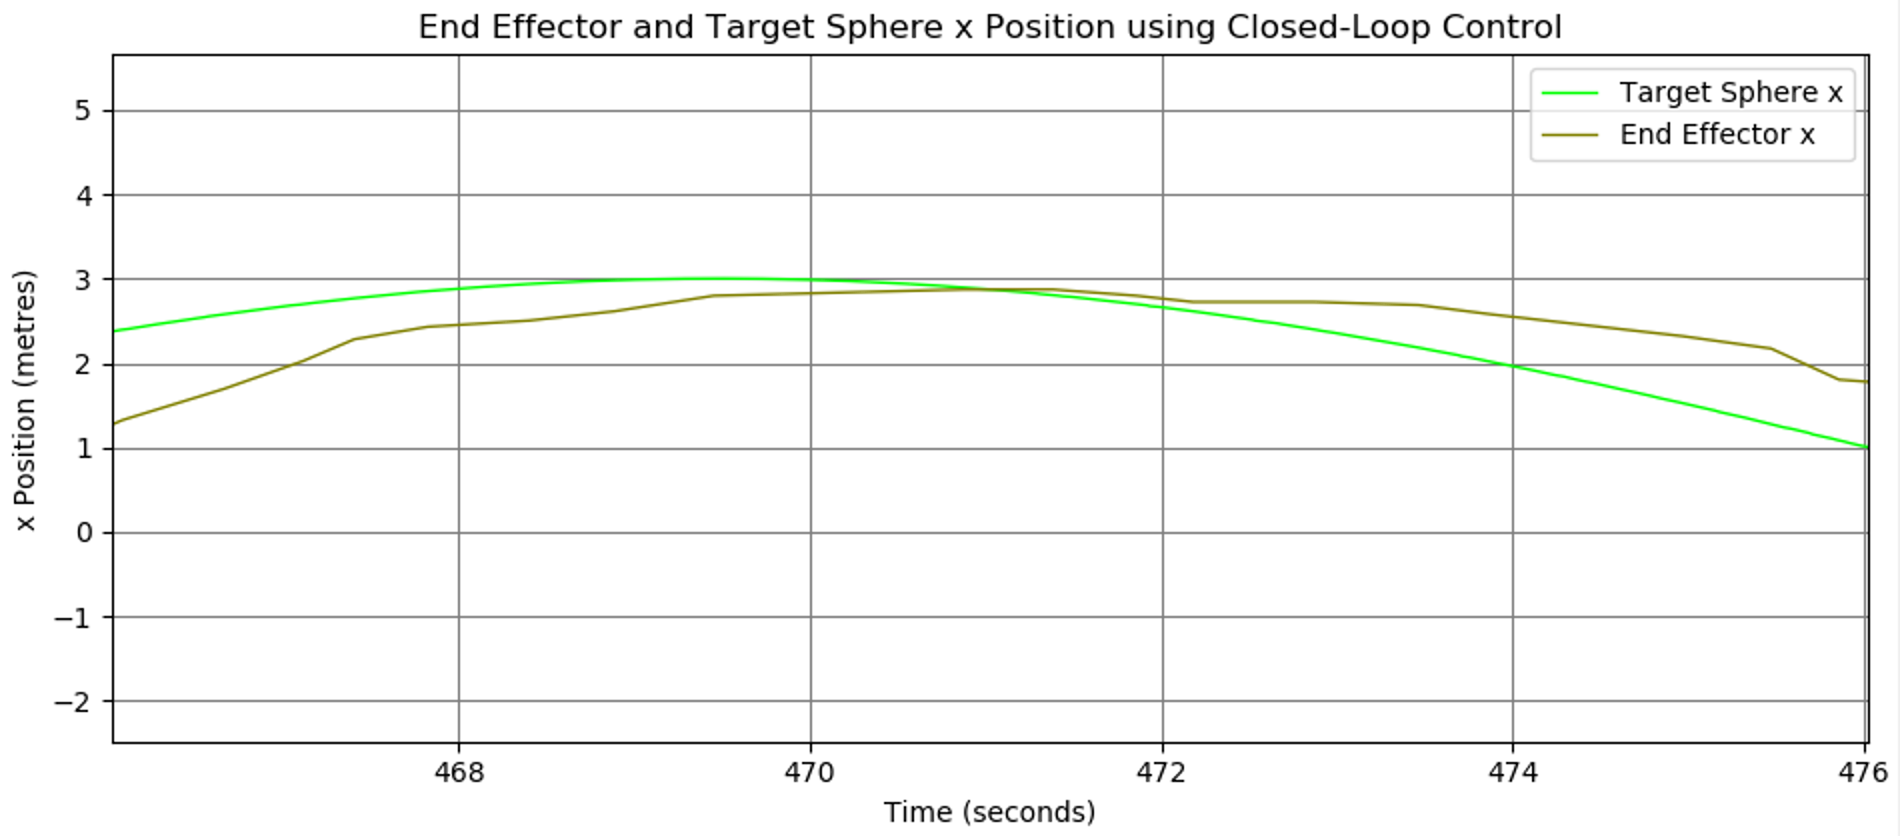
\includegraphics[width=0.4\textwidth]{images/3.2x.png}
        &
        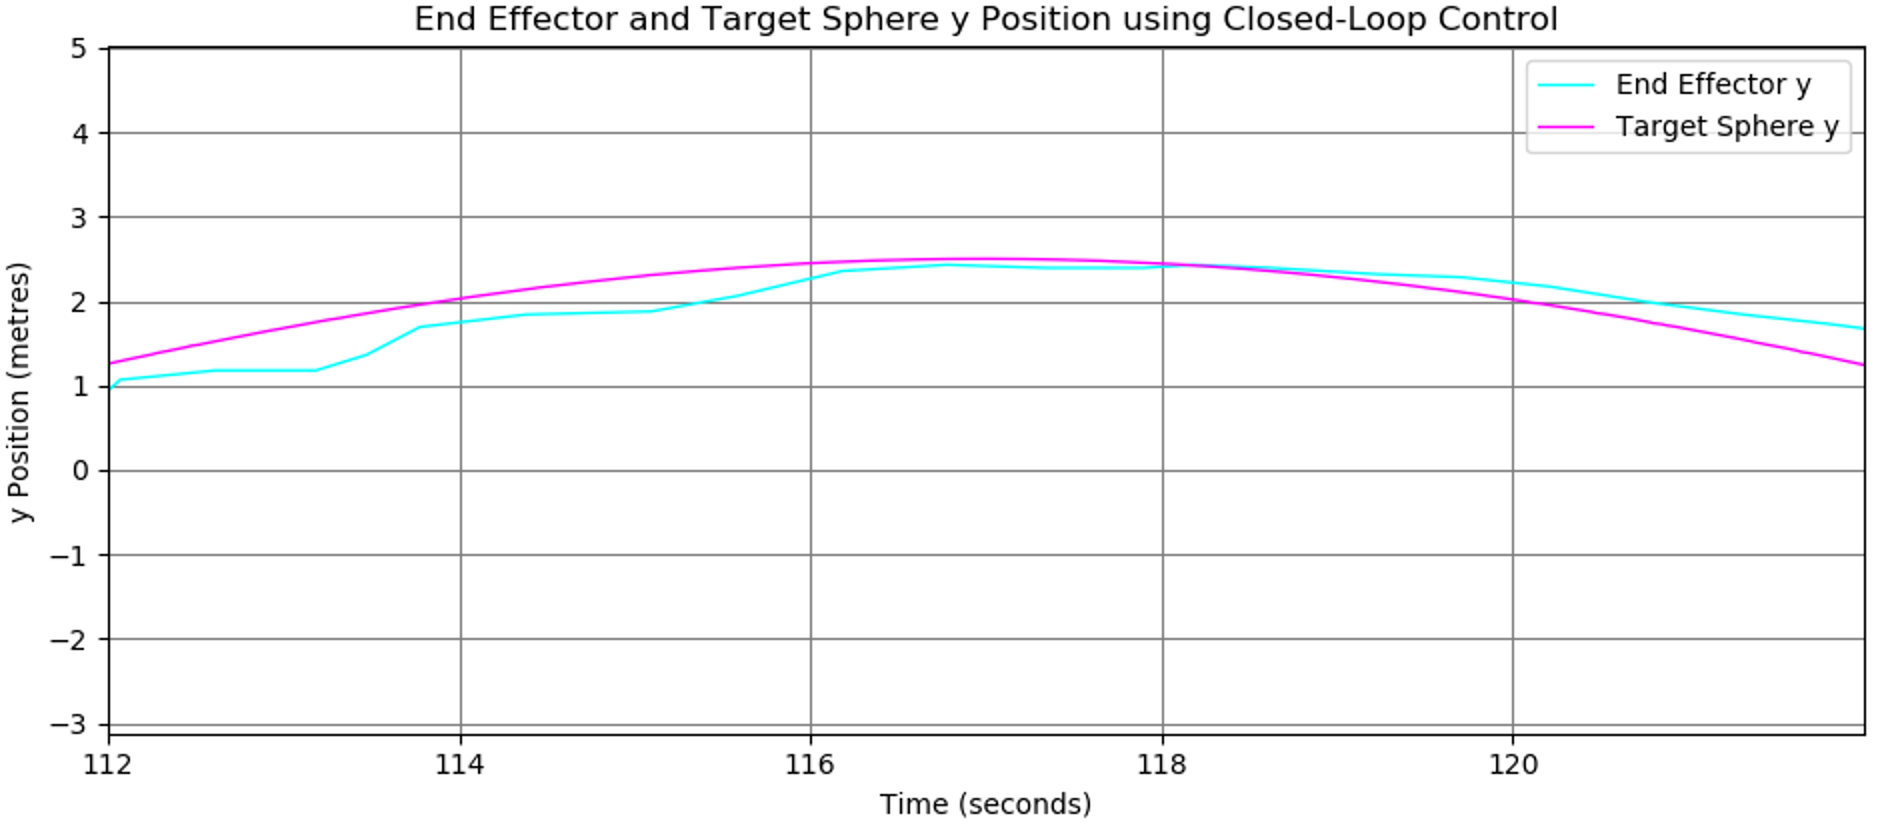
\includegraphics[width=0.4\textwidth]{images/3.2y.png}
    \end{tabular}
    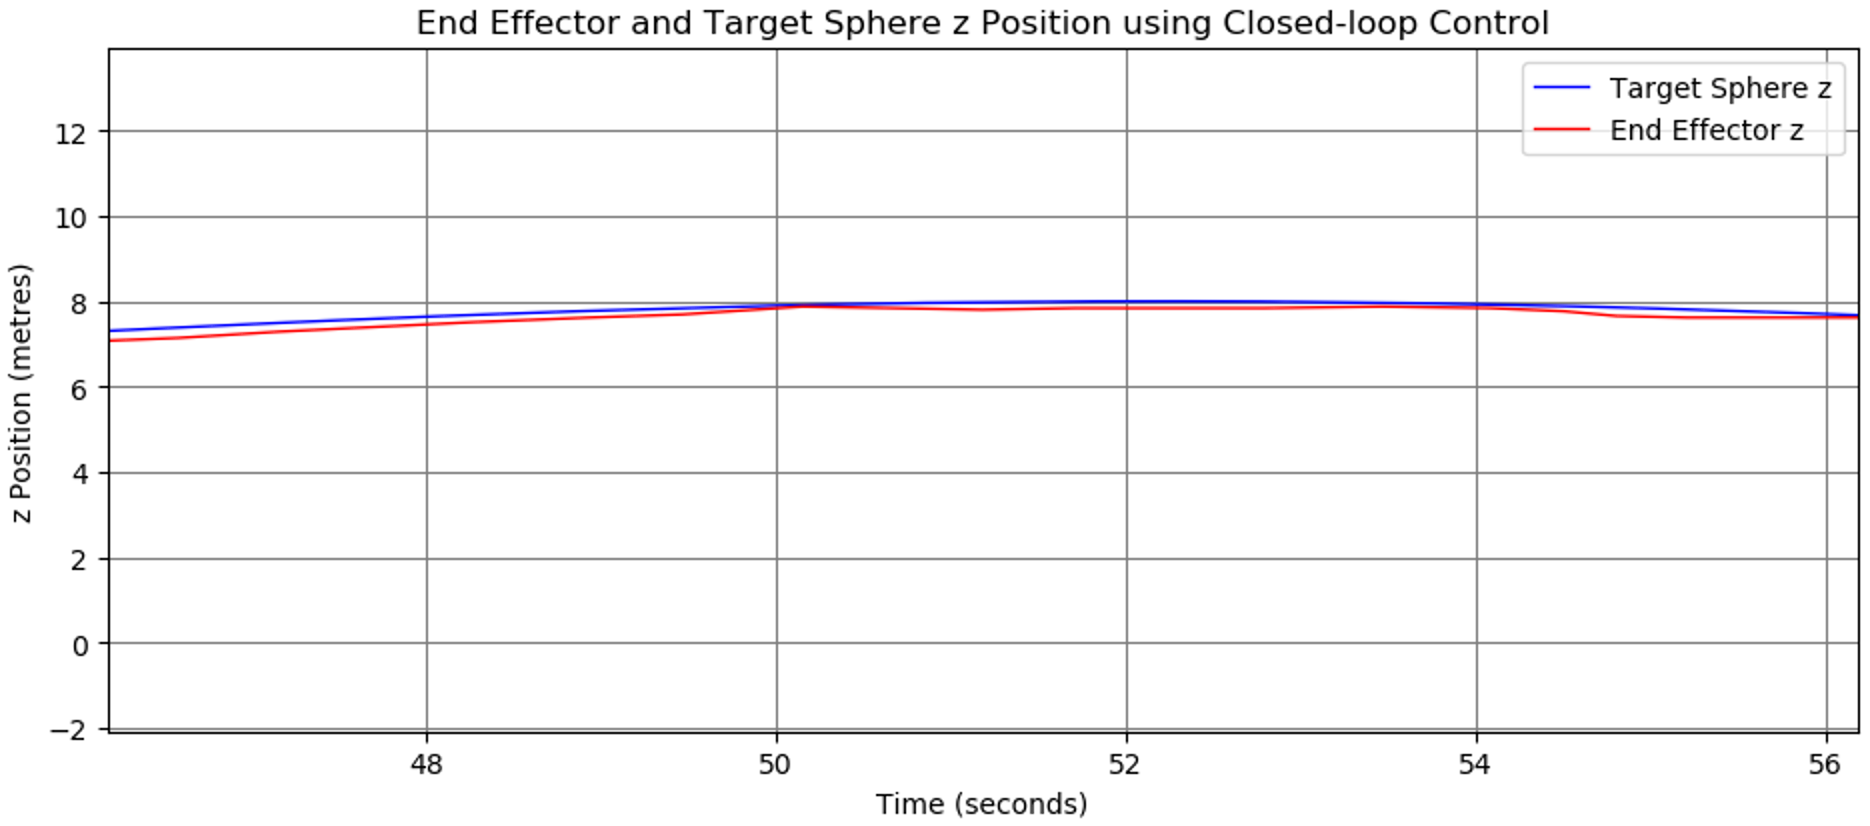
\includegraphics[width=0.4\textwidth]{images/3.2z.png}
\end{center}

\section{Final Task}
\setcounter{subsection}{1}
\subsection{Null-space Control}

\begin{center}
    \begin{tabular}{ll}
        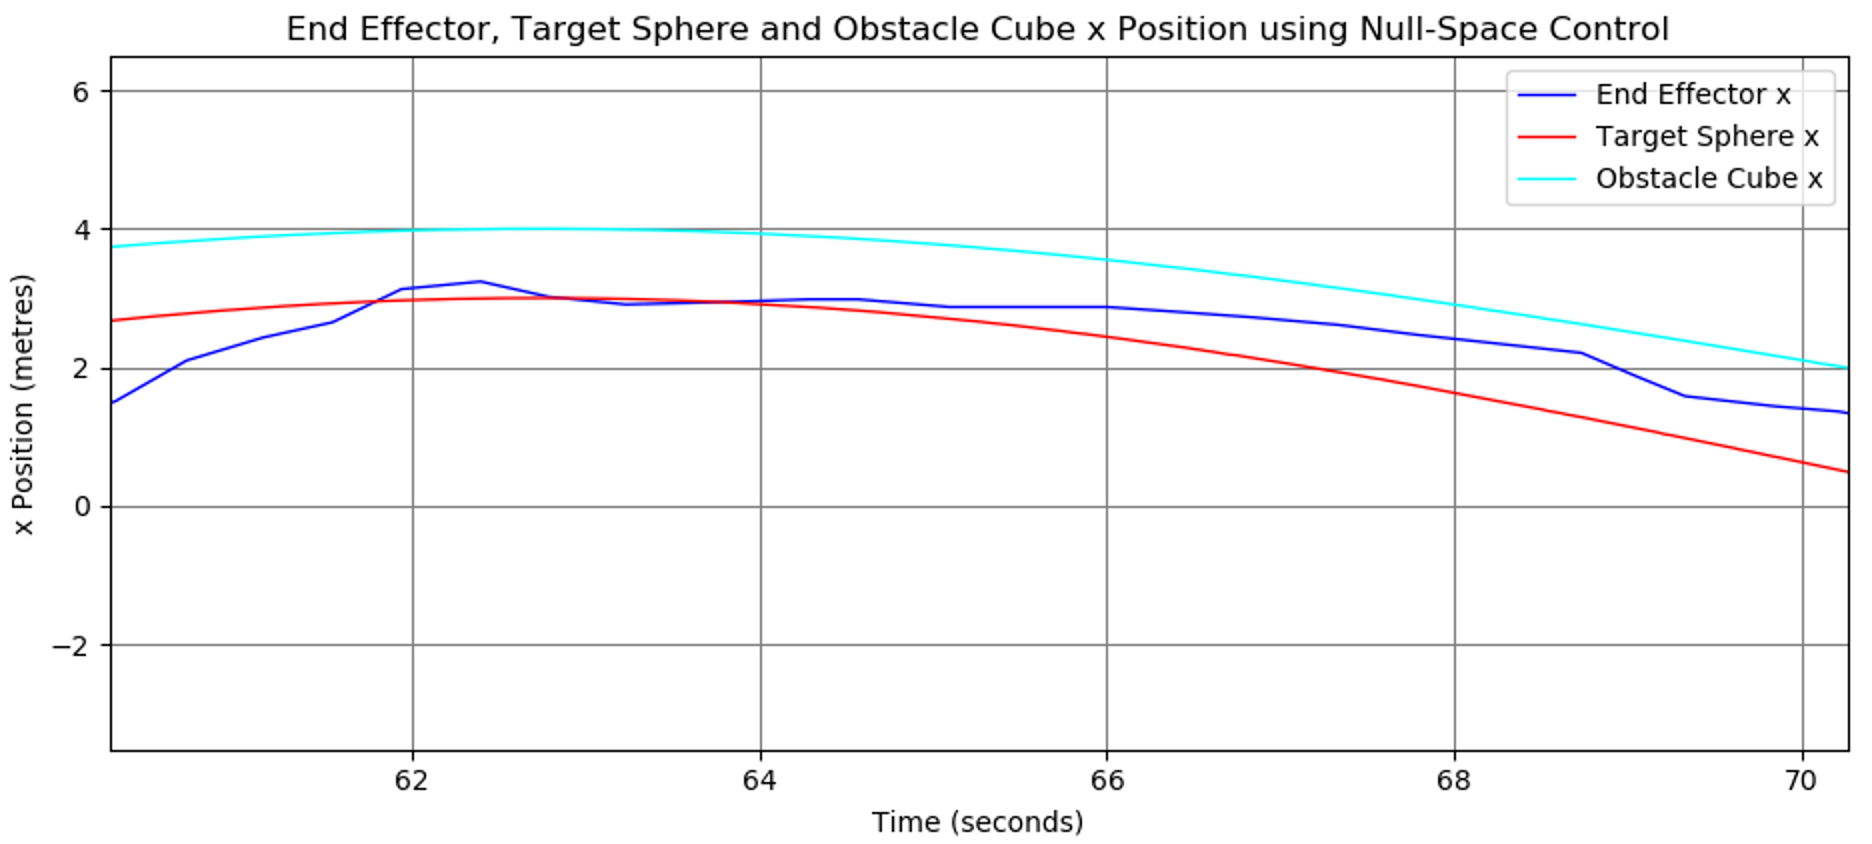
\includegraphics[width=0.4\textwidth]{images/nullspace_x.png}
        &
        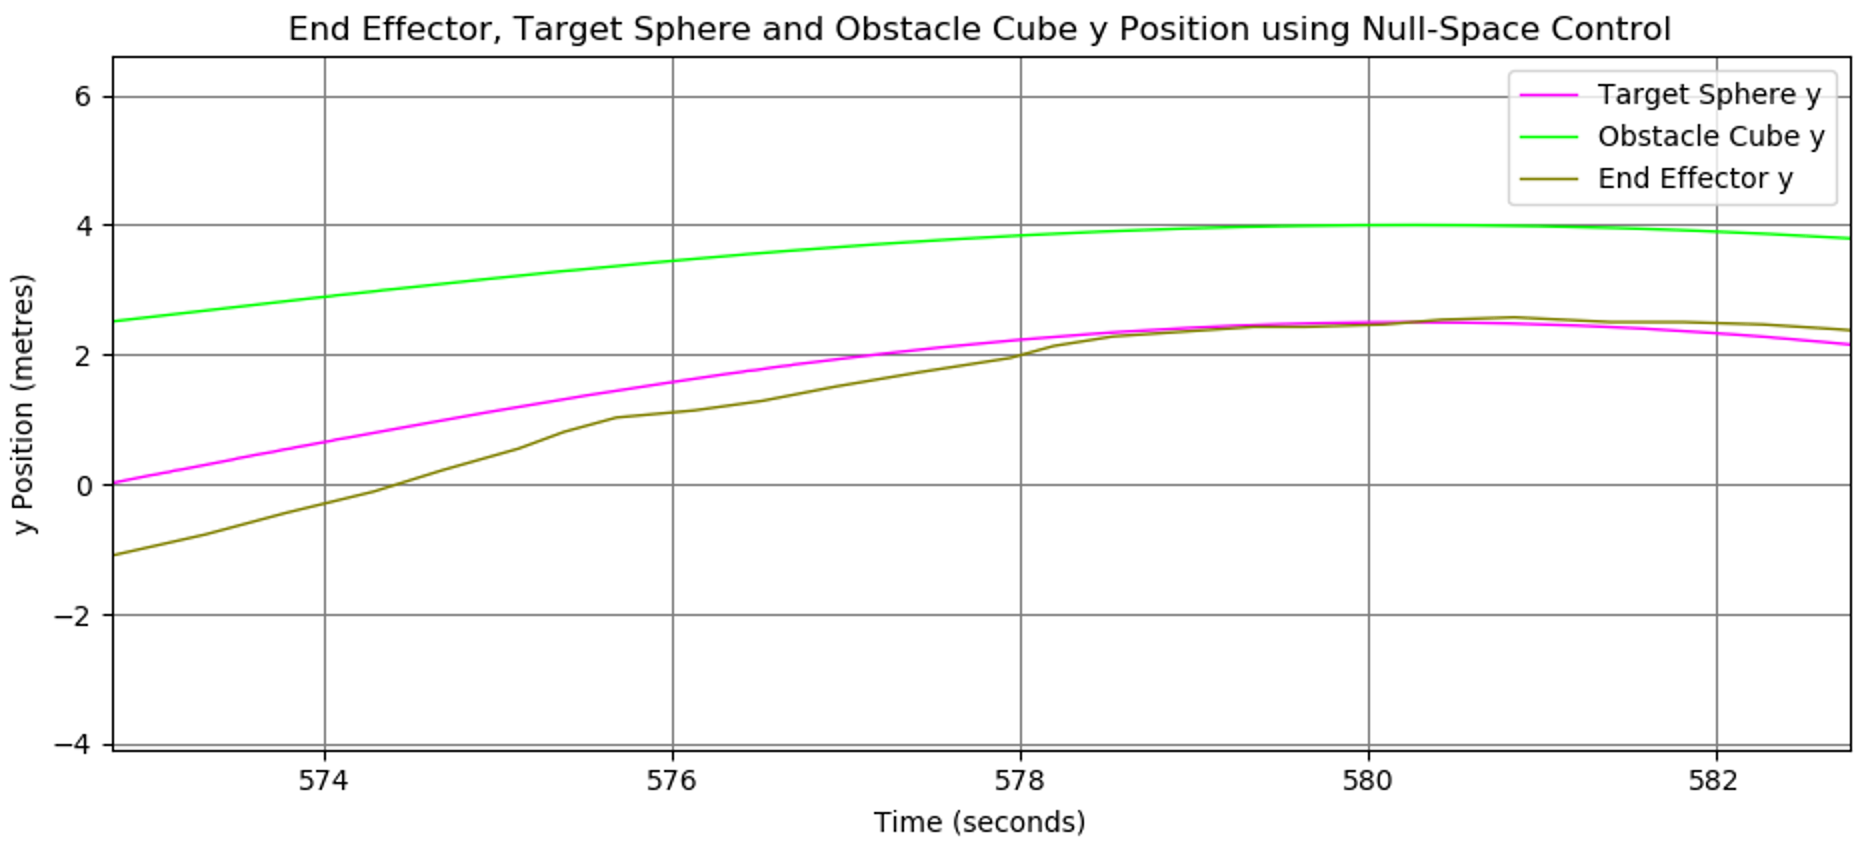
\includegraphics[width=0.4\textwidth]{images/nullspace_y.png} \\
        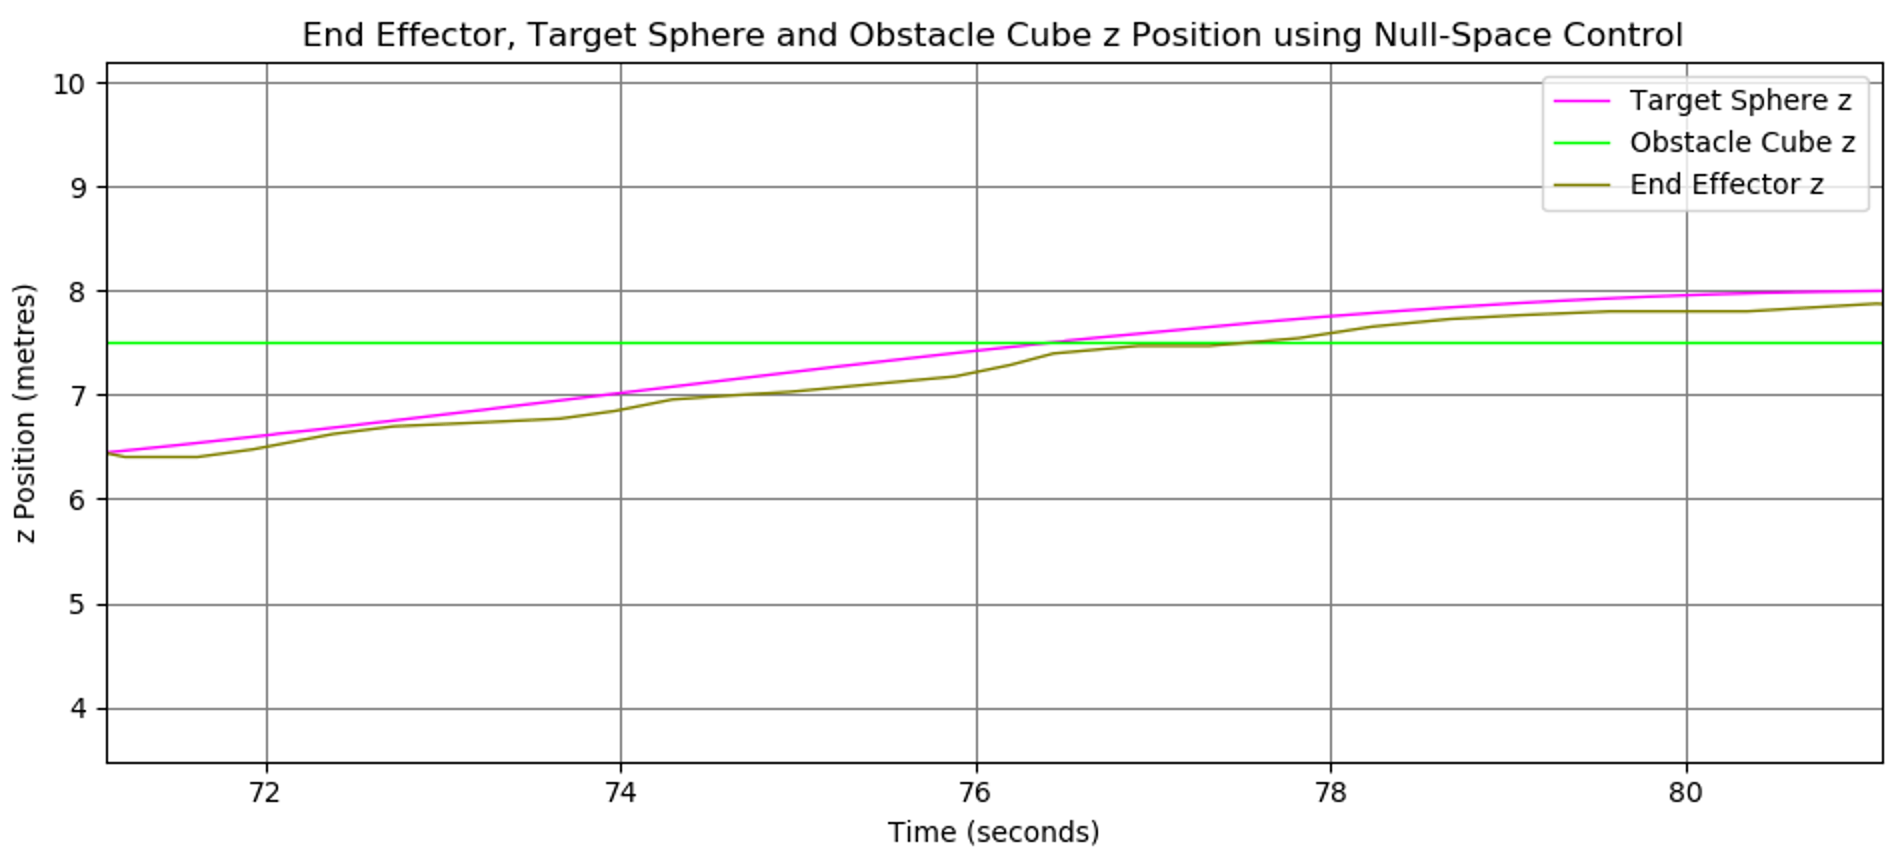
\includegraphics[width=0.4\textwidth]{images/nullspace_z.png} & 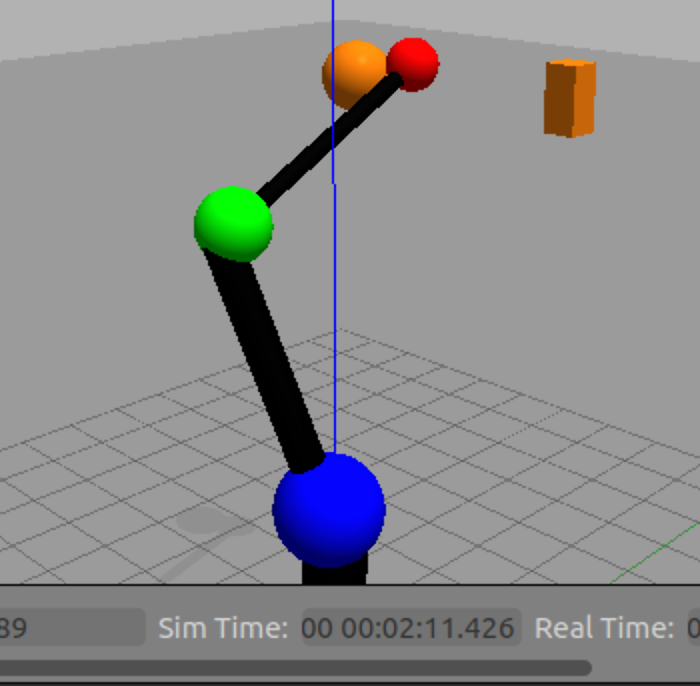
\includegraphics[height=0.18\textwidth]{images/nullspace_pic.png}
    \end{tabular}
\end{center}

The previous closed-loop controller attempted to move the robot end effector to track the spherical target as closely as possible. This null-space controller is similar in that it also attempts to track the spherical target, but has a secondary goal of attempting to avoid hitting the cube target as much as possible without compromising the original goal of tracking the spherical target.

Our robot is a redundant system: it has more DOF than is needed to complete the task of tracking the sphere. This is because both joint 2 and joint 4 rotate around the \(x\) axis, meaning we can achieve the same end effector position using two different sets of angles for these joints (at least for the task of positioning the end effector close to the sphere - the robot may not be redundant in other tasks such as moving to extreme positions). In other words, it is possible to accomplish our primary goal of tracking the spherical target with multiple joint configurations.

Using this knowledge, we can also send control signals to achieve our secondary goal of avoiding the cube target without affecting the performance of our primary goal. This is done by creating a secondary controller for our secondary goal, that operates in the null space of the primary controller for our primary goal. The final control signal sent to the robot is the sum of the control signal from the primary controller, and a filtered version of the control signal from the secondary controller. In general, this is a technique that can be applied with further controllers as well, but in this case we only have two.

Our final control signal \(\pmb{\tau}\) is defined as such: \[\pmb{\tau} = \pmb{\tau_1} + N(\pmb{q})\pmb{\tau_2}\] where \(\pmb{\tau_i}\) represents the control signal from the controller for the \(i\)th priority goal.

\(N(\pmb{q})\) is the null space projector that projects a given vector into the null space of the primary goal. \(N(\pmb{q})\) is defined as follows: \[N(\pmb{q}) = I - J(\pmb{q}) \bar{J}(\pmb{q})\] where \(\bar{J}\) is the pseudo-inverse of the Jacobian. This means that the control signal \(\pmb{\tau_2}\) from our seconday controller will be subtracted from itself everywhere that affects the primary operational space movement, and is left to apply any control signal that is in the null space of the primary controller.

The controller for our seconday goal is responsible for ensuring the robot stays as far from the cube target as possible. This is done by attempting to maximize the distance between joint 4 (green joint) and the cube target. The distance from joint 4 is maximized as this is the joint that can be moved in three dimensional space without affecting the end effector position, due to the redundancy of our robot. As explained earlier, the control signal from this controller for our seconday goal is then projected into the null space of the primary controller, meaning any control signal left after this projection does not affect our primary goal. An example of this effect can be seen in the screenshot of our robot above, where the end effector is tracking the sphere as closely as it can, but joint 4 is positioned to be as far away from the cube target as possible.

\end{document}
